\section{模型评估与选择}
\subsection{经验误差与过拟合}
\subsubsection{经验误差}

通常我们把分类错误的样本数占样本总数的比例称为"\textbf{错误率}"(error rate),即如果在 $m$ 个样本中,有$a$个样本错误,则错误率:
\[E=\frac{a}{m}\]

相应的,也有\textbf{精度}(accuracy):
\[A = 1-\frac{a}{m}\]

我们把学习器的实际预测输出与样本的真实输出之间的差异称为``误差",学习器在训练集上的误差称为``训练误差"或``\textbf{经验误差}"(empirical error),在新样本上的误差称为``\textbf{泛化误差}"(generalization error)。

\subsubsection{过拟合}

当学习器将训练样本训练得太好的时候,往往会将一些特异点当作一般性质,这样会导致模型的泛用性下降,在新样本上表现不好,这种现象在机器学习中称为``过拟合"(overfitting)。与过拟合相对的也有``欠拟合"(underfitting)。欠拟合问题很好解决,而过拟合则是机器学习的一大障碍。

\subsection{评估方法}

通常我们会选定一个\textbf{测试集}来测试学习器对新样本的判别能力,然后以测试集上的``测试误差"作为泛化误差的近似。需要注意的是\textbf{测试集应尽可能与训练误差互斥,即测试样本尽量不在训练集中出现,未在训练集中使用过。}

一个数据集可以通过适当的处理,从中产生出训练集 $S$ 和测试集 $T$。

\subsubsection{留出法}

``留出法''(hold-out) 直接将数据集$D$划分成两个互斥的集合:训练集 $S$,测试集$T$。有 $D = S \cup T,S\cap D = \varnothing$。在 $S$ 上训练出模型后,用 $T$ 来评估期测试误差。

单次使用留出法往往是不够稳定可靠的,一般采用若干次随即划分,重复实验后取平均值作为评估结果。

常常将 2/3 - 4/5 的样本用于训练,剩余样本用于测试。

\subsubsection{交叉验证法}

``交叉验证法''(cross validation)先将数据集 $D$ 划分为 $k$ 个大小相似的互斥子集,即 $D = D_1 \cup D_2 \cup \cdots \cup D_k,D_i \cap D_j = \varnothing (i\neq j)$,每个子集都尽可能保证数据分布一致性,即从$D$中分层采样\footnote{先将总体的单位按某种特征分为若干次级总体(层),然后再从每一层内进行单纯随机抽样,组成一个样本。}得到。然后,每次用 $k-1$ 个子集的并集作为训练集,余下的那个子集作为测试集;这样可获得 $k$ 组训练/测试集,从而进行 $k$ 次实验,最终返回的是 $k$ 个测试结果的均值。

交叉检验法评估结果的稳定性和保真性很大程序上取决于 $k$ 的取值,为强调这一点,通常把交叉检验法称为``$k$折交叉检验''。$k$ 最常用取值为10,其他也常用5,20。

\begin{figure}[H]
    \centering
    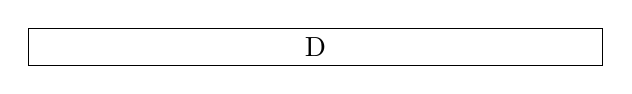
\begin{tikzpicture}[scale = 1]
        \node [draw,inner xsep = 10em] {D};
    \end{tikzpicture}
    \caption{10折交叉检验示意图}
    \label{10折交叉检验示意图}
\end{figure}

与留出法类似,将数据集 $D$ 划分为 $k$ 个子集存在多种划分方式。为减小因样本划分不同而引入的差别,$k$折交叉验证通常要随机使用不同的划分重复 $p$ 次,最终的评估结果是这 $p$ 次 $k$ 这交叉检验结果的均值。常见的有 ``10次10折交叉检验''。

假定数据集 $D$ 中有 $m$ 个样本,若 $k=m$,则得到了交叉检验法的一个特例:留一法。留一法的训练结果往往比较准确,但在数据极大的情形下,考虑到算法开销,并不是十分适用。

\subsubsection{自助法}

我们希望评估的是用 $D$ 训练出的模型,但在留出法和交叉检验中,由于保留了一部分样本用于测试,因此实际评估的模型所使用的训练集比 $D$ 小。而留一法又因为计算复杂度太高,往往难以接受。

``自助法''(bootstrapping) 直接以自助采样法\footnote{有放回地采样}为基础。给定包含 $m$ 个样本的数据集 $D$,我们对它进行采样产生数据集 $D^{'}$:每次随机从 $D$ 中挑选一个样本,将其拷贝放入 $D^{'}$,然后再将该样本放回初始数据集 $D$ 中,使得该样本在下次采样时仍有可能被采到;这个过程重复执行 $m$ 次后,我们就得到了包含 $m$ 个样本的数据集 $D^{'}$。

显然,$D$中有一部分样本会在 $D^{'}$中多次出现,而另一部分样本不出现。样本在 $m$ 次采样中始终不被采到地概率是:

\begin{equation}
    \lim_{m\rightarrow\infty}(1-\frac{1}{m})^m = \frac{1}{e} = 0.368
\end{equation}
即通过自助采样,初始数据集中约有 36.8\% 的样本未出现在采样数据集$D^{'}$中。于是我们可以将 $D^{'}$ 作为训练集。

自助法在数据量较小,难以有效划分训练/测试集时很有用;然而,自助法产生的数据集改变了数据集的分布,这回引入估计偏差。因此,在初始数据量足够时,留出法和交叉检验法更常用一些。

\subsubsection{调参与最终模型}

大多数学习算法都有些参数(parameter)需要设定,参数配置不同,学得模型的性能往往有显著差别。

调参时需要注意,参数往往实在实数范围内取值,因此,对每种参数配置都训练出模型来是不可行的。现实中常用的做法是对每个参数选定一个\textbf{范围}和变化\textbf{步长},例如 [0,0.2] 范围内以 0,05 为步长,则实际要评估的候选参数值就有 5 个,最终结果在折 5 个值中产生。显然这不是最佳结果,但却是在计算开销和性能估计之间的折中值。

在给定包含 $m$ 个样本的数据集 $D$,在模型评估与选择过程中由于需要流出一部分数据进行评估测试,事实上,我们只使用了一部分数据训练模型。因此,在模型选择完成后,学习算法和参数配置已旋定,此时应该用数据集$D$重新训练模型。这个模型在训练过程中使用了所有 $m$ 个模型,这才是最终的模型。

我们通常把学得模型在实际使用中遇到的数据称为测试数据,为了加以区别,模型评估与选择中用于评估测试的数据集常称为``验证集''(validation set)。

\subsection{性能度量}

性能度量是指对模型泛化能力的评价。性能度量反映了任务需求,在对比不同模型的能力时,使用不同的性能度量往往会导致不同的评判结果。这也意味着模型的``好坏''是相对的。

在预测任务中,给定样例集 $D=\{(\bm{x}_1,y_1),(\bm{x}_2,y_2),\cdots,(\bm{x}_m,y_m)\}$。其中 $y_i$ 是真实标记。评估学习器 $f$ 的性能,就要把学习器预测结果 $f(\bm{x})$ 与真是标记 $y$ 进行比较。

回归任务最常用的性能度量是``均方误差'':
\begin{equation}
    E(f;D) = \frac{1}{m}\sum_{i=1}^{m}(f(\bm{x}_i)-y_i)^2
\end{equation}

更一般的,对于数据分布 $\mathcal{D}$ 和概率密度函数 $p(\cdot)$,均方误差可描述为:
\begin{equation}
    E(f;D) = \int_{x\sim D}(f(\bm{x})-y)^2p(\bm{x})\text{d}\bm{x}
\end{equation}

\subsubsection{错误率与精度}

错误率是分类错误的样本占样本总数的比例,精度则相反。错误率定义:

\begin{equation}
    E(f;D) = \frac{1}{m}\sum_{i=1}^m \mathbb{I} (f(\bm{x}_i)\neq y_i)
\end{equation}

精度定义:

\begin{equation}
    \begin{aligned}
        E(f;D) & = \frac{1}{m}\sum_{i=1}^m \mathbb{I} (f(\bm{x}_i) = y_i) \\
               & = 1 - E(f;D)
    \end{aligned}
\end{equation}

更一般地,对于数据分布 $\mathcal{D}$ 和概率密度函数 $p(\cdot)$,错误率和精度有如下定义:
\begin{equation}
    E(f;\mathcal{D}) = \int_{x\sim D} \mathbb{I} (f(\bm{x})\neq y)p(\bm{x})\text{d}\bm{x}
\end{equation}
\begin{equation}
    \begin{aligned}
        acc(f;\mathcal{D}) & = \int_{x\sim D} \mathbb{I} (f(\bm{x})= y)p(\bm{x})\text{d}\bm{x} \\
                        & = 1 - E(f;\mathcal{D})
    \end{aligned}
\end{equation}

\subsubsection{查准率,查全率与F1}

对于二分类问题,可以将样例根据其真是类别与学习器预测类别的组合划分为真正例(true positive),假正例(false positive),真反例(true negative),假反例(false negative)四种情形,令 TP,FP,TN,FN 分别表示其对应的样例数,显然有 TP+FP+TN+FN=样例总数。

\begin{table}[H]
    \centering
    \caption{分类结果混淆矩阵}
    \label{table:分类结果混淆矩阵}
    \setlength{\tabcolsep}{7mm}
    \begin{tabular}{c|c|c}
        \toprule
        \multirow{2}{*}{\textbf{真实情况}} &  \multicolumn{2}{c}{\textbf{预测结果}} \\ \cline{2-3}
        & 正例 & 反例  \\ 
        \midrule
        正例 & TP(真正例) & FN(假反例) \\
        反例 & FP(假正例) & TN(真反例) \\
        \bottomrule
    \end{tabular}
\end{table}

准确率/查准率,即预测结果为正例且正确的比例:
\begin{equation}
    P = \frac{TP}{TP+FP}
\end{equation}

召回率/查全率,即正例被预测出的比例:
\begin{equation}
    R = \frac{TP}{TP+FN}
\end{equation}

查准率与查全率是一对矛盾的度量,一般来说,查准率高时,查全率往往比较低;反之亦然。我们以查准率为纵轴,查全率为横轴作图,就得到了查准率-查全率曲线,简称``P-R图"

\begin{figure}[H]
    \centering
    \begin{tikzpicture}[scale = 1]
        \draw [name = x,thick] (0,0) -- (5,0) node(xline) {} node [node font = \footnotesize,below = 10pt,pos = 0.5] {查全率};
        \draw [name = y,thick] (0,0) -- (0,5) node(yline) {} node [node font = \footnotesize,left = 22pt,pos = 0.6,rotate = 90] {查准率};
        \foreach \x/\y in {0/0,0.2/1,0.4/2,0.6/3,0.8/4,1.0/5}
            \draw [thick] (0,\y) -- (0.1,\y) node[anchor = east] {\footnotesize$\x$};
        \foreach \x/\y in {0.2/1,0.4/2,0.6/3,0.8/4,1.0/5}
            \draw [thick] (\y,0) -- (\y,0.1) node[anchor = north] {\footnotesize$\x$};
        \draw [color = red,name path = A] (0,5) ..controls (5,5) and (4.5,2) .. (5,0) node [anchor = south,node font = \footnotesize,pos = 0.2] {A};
        \draw [name path = B] (0,5) ..controls (3,4) and (5,4) .. (5,0) node [anchor = west,node font = \footnotesize,pos = 0.8] {B};
        \draw [name path = C] (0,5) ..controls (3,4) and (4.5,2) .. (5,0) node [anchor = north,node font = \footnotesize,pos = 0.2] {C};
        \draw [name path = M,dashed,color = red] (0,0) -- (4.5,4.5);
        \draw [fill,red,name intersections = {of = A and M}] (intersection-1) circle (2pt) node(1) {};
        \draw [fill,red,name intersections = {of = B and M}] (intersection-1) circle (2pt) node(2) {};
        \draw [fill,red,name intersections = {of = C and M}] (intersection-1) circle (2pt) node(3) {};
        \draw [red,dotted] (1) -- (1|-xline) (2) -- (2|-xline) (3) -- (3|-xline);
        \draw [red,dotted] (1) -- (1-|yline) (2) -- (2-|yline) (3) -- (3-|yline);
        \node [red,node font = \footnotesize] (text) at (3.5,4.8) {平衡点};
        \draw [->,>=Stealth,color = red!50] (text) -> (1);
        \draw [->,>=Stealth,color = red!50] (text) -> (2);
        \draw [->,>=Stealth,color = red!50] (text) -> (3);
    \end{tikzpicture}
    \caption{P-R曲线与平衡点示意图}
    \label{P-R曲线与平衡点示意图}
\end{figure}   

若一个学习器的 P-R 曲线被另一个学习器的曲线完全``包住'',则可断言后者的性能优于前者,如上图的学习器 A 优于学习器 C。如果两个学习器发生了交叉,如学习器 A 和 B ,则很难断言两者孰优孰劣。只能在具体的查准率或查全率条件下进行比较。然而,在很多情形下,人们希望比较学习器 A 和 B,则可以通过曲线下面积的大小比较,它在一定程度上表征了学习器在查准率和查全率上取得相对``双高''的比例。但是这个值不太容易估算,因此会采用一些替代的方法度量。

``平衡点''(Break-Even Point,检查 BEP)是``查准率=查全率''时的取值,可以通过这点对应的查全率(或查准率)进行比较。

但 BEP 还是过于简化了,更常用的是 $F1$ 度量\footnote{$F1$ 是基于调和平均数定义的:$\frac{1}{F1} = \frac{1}{2} \cdot (\frac{1}{P} + \frac{1}{R})$}。
\begin{equation}
    F1 = \frac{2\times P \times R}{P+R} = \frac{2 \times TP}{\text{样例总数} + TP - TN}
\end{equation}

在一些应用中,对查准率和查全率的重视程度有所不同、此时我们需要 $F1$ 度量的一般形式 $F_\beta$ 度量\footnote{ $F_\beta$ 是基于加权调和平均数定义的:$\frac{1}{F_{\beta}} = \frac{1}{1+\beta ^ 2} \cdot (\frac{1}{P} + \frac{\beta ^2}{R})$}:
\begin{equation}
    F_{\beta} = \frac{(1+\beta^2)\times P \times R}{(\beta ^ 2 \times P) + R}
\end{equation}
其中 $\beta>0$ 度量了查全率对查准率的相对重要性。$\beta = 1$ 时退化为 $F1$; $\beta > 1$ 时查全率有更大影响;$\beta <1$ 时查准率有更大影响。

一种直接的做法是先在各混淆矩阵上分别计算出查准率与查全率,记为 $(P_1,R_1),(P_2,R_2),$\\
$\cdots,(P_n,R_n)$,再计算平均值,这样就得到``宏查准率''(macro-P),``宏查全率''(macro-R),以及相应的``宏F1''(macro-F1)

\begin{align}
    marco-P =& \frac{1}{n}\sum_{i=1}^n P_{i} \\
    marco-R =& \frac{1}{n}\sum_{i=1}^n R_{i} \\
    marco-F1 =& \frac{ 2\times macro-P \times macro-R }{ macro-R + macro-R } 
\end{align}

还可以先将各混淆矩阵的对应元素进行平均,得到 $TP,FP,TN,FN$ 的平均值 $\overline{TP},\overline{FP},\overline{TN},\overline{FN}$ 再基于这些平均值计算出 ``微查准率''(micro-P),``微查全率''(micro-R),以及相应的``微F1''(micro-F1)

\begin{align}
    micro-P =& \frac{\overline{TP}}{\overline{TP} + \overline{FP}} \\
    micro-R =& \frac{\overline{TP}}{\overline{TP} + \overline{FN}} \\
    micro-F1 =& \frac{ 2\times macro-P \times macro-R }{ macro-R + macro-R } 
\end{align}

\subsubsection{ROC 与 AUC}

很多学习器是为测试样本产生一个实值或概率预测,然后将这个预测值与一个分类阈值(threshold)进行比较,若大于阈值则为正类,否则为反类。这个实质或概率预测结果的好坏,直接决定了学习器的泛化能力。实际上,根据这个实值或概率预测的结果,我们可将测试样本进行排序,``最可能''是正例排在最前面,``最不可能''是正例排在最后面。这样,分类过程就相当于在这个排序中以某个``截断点''将样本分成了两部分,前一部分判作正例,后一部分判作反例。

在不同的应用任务中,我们可根据任务需求不同采用不同的截断点,例如若我们更中式``查准率'',则可选择排序中靠前的位置进行截断。因此,排序本身的质量好坏,体现了综合考虑学习器在不同任务下的``期望泛化性能''的好坏。ROC 曲线则是从这个角度出发来研究学习器泛化性能的有力工具。

ROC 全称``受试者工作特征''曲线,与 P-R 曲线类似,根据学习器的预测结果对样例进行排序,按此顺序逐个把样本作为正例进行预测,每次计算出两个重要量的值,分别以它们为横纵坐标作图,就得到了 ``ROC 曲线''。ROC 曲线的纵轴是 ``真正例率''(True Positive Rate,简称 TPR),横轴是 ``假正例率''(False Positive Rate,简称 FPR),两者定义为:

\begin{align}
    TPR = \frac{TP}{TP+FN} \\
    FPR = \frac{FP}{TN+FP} 
\end{align}

下图给出了一个示例,显然,对角线对应于 ``随即猜测'' 模型,而点(0,1)则对应于将所有正例排在所有反例之前的``理想模型''。

\begin{figure}[H]
    \centering
    \begin{minipage}{0.4\linewidth}
        \begin{tikzpicture}[thick,node font = \footnotesize]
            \draw (0,0) rectangle (5,5);
            \foreach \x/\y in {0/0,1/0.2,2/0.4,3/0.6,4/0.8,5/1.0}
                \draw (0,\x) -- (0.1,\x) node [left = 5pt] {\y};
            \foreach \x/\y in {1/0.2,2/0.4,3/0.6,4/0.8,5/1.0}
                \draw (\x,0) -- (\x,0.1) node [below = 5pt] {\y};
            \node at (2.5,-0.7) {假正确率};
            \node at (-0.9,2.5) [rotate = 90] {真正确率};
            \draw [fill=gray!20] (5,0) -- (0,0) ..controls (1,4) and (4,5) .. (5,5) node [pos = 0.4,above=0.5cm] {ROC曲线} -- (5,0);
            \draw [dashed] (0,0) -- (5,5) node [pos = 0.6,below=1cm] {AUC};
        \end{tikzpicture}
        \caption{ROC 与 AUC}
        \label{ROC 与 AUC}
    \end{minipage}
    \begin{minipage}{0.4\linewidth}
        \begin{tikzpicture}[thick,node font = \footnotesize]
            \draw (0,0) rectangle (5,5);
            \foreach \x/\y in {0/0,1/0.2,2/0.4,3/0.6,4/0.8,5/1.0}
                \draw (0,\x) -- (0.1,\x) node [left = 5pt] {\y};
            \foreach \x/\y in {1/0.2,2/0.4,3/0.6,4/0.8,5/1.0}
                \draw (\x,0) -- (\x,0.1) node [below = 5pt] {\y};
            \node at (2.5,-0.7) {假正确率};
            \node at (-0.9,2.5) [rotate = 90] {真正确率};
            \draw [fill=gray!20] (0,0.5)--(0.25,0.5)--(0.25,1)--(0.5,1)--(0.5,1.25)--(1,1.25)--(1,1.5)--(1.25,1.5)--(1.25,2)--(1.25,2)--(1.5,2)--(1.75,2)--(2,2)--(2,2.25)--(2,2.5)--(2.75,2.5)--(2.75,3)--(3,3)--(3.25,3)--(3.25,3.25)--(3.25,3.75)--(3.5,3.75)--(3.5,4)--(4,4)--(4.25,4)--(4.25,4.5)--(5,4.5)--(5,5)--(5,0)--(0,0);
            \fill (0,0.5) circle (1.5pt) (0.25,0.5) circle (1.5pt) (0.25,1) circle (1.5pt) (0.5,1) circle (1.5pt) (0.5,1.25) circle (1.5pt) (1,1.25) circle (1.5pt) (1,1.5) circle (1.5pt) (1.25,1.5) circle (1.5pt) (1.25,2) circle (1.5pt) (1.25,2) circle (1.5pt) (1.5,2) circle (1.5pt) (1.75,2) circle (1.5pt) (2,2) circle (1.5pt) (2,2.25) circle (1.5pt) (2,2.5) circle (1.5pt) (2.75,2.5) circle (1.5pt) (2.75,3) circle (1.5pt) (3,3) circle (1.5pt) (3.25,3) circle (1.5pt) (3.25,3.25) circle (1.5pt) (3.25,3.75) circle (1.5pt) (3.5,3.75) circle (1.5pt) (3.5,4) circle (1.5pt) (4,4) circle (1.5pt) (4.25,4) circle (1.5pt) (4.25,4.5) circle (1.5pt) (5,4.5) circle (1.5pt);
            \node at (3,2) {AUC};
        \end{tikzpicture}
        \caption{基于有限样例的 ROC 曲线与 AUC}
        \label{基于有限样例的 ROC 曲线与 AUC}
    \end{minipage}

\end{figure}

现实中往往不能产生光滑曲线,只能产生近似 ROC 曲线。绘制过程如下:给定 $m^{+}$ 个正例和 $m^{-}$ 个反例。根据学习器预测结果对样例进行排序,然后把分类阈值设为最大,即把所有样例预测为反例,此时真正利率和假正例率均为0,在坐标(0,0)处标记一个点。然后,将分类阈值依次设为每个样例的预测值,即依次将每个样例划分为正例。设前一个标记点坐标为 (x,y),当前若为真正例,则对应标记点的坐标为 $(x,y+\frac{1}{m^+})$;当前若为假正例,则对应标记点的坐标为 $(x+\frac{1}{m^-},y)$,然后用线段连接相邻点即得。

进行学习器的比较时,与 P-R 曲线类似,若一个学习器的 ROC 曲线完全被另一个学习器的曲线 ``包住'' 则可断言后者的性能由于前者;若两个学习器的 ROC 曲线发生交叉,则难以断言。此时若一定需要断言,则可以通过比较 ROC 曲线下方的面积,即 AUC(Area Under ROC Curve)。

从定义可知,AUC 可通过对 ROC 曲线下各部分的面积求和而得。假设 ROC 曲线是由坐标 $(x_i,y_i)$ 点组成的,则 AUC 可估算为:
\begin{equation}
    AUC = \frac{1}{2}\sum_{i=1}^{m-1}(x_{i+1}-x_i)\cdot(y_i+y_{i+1})
\end{equation}

形式化地看,AUC 考虑的是样本预测的排序质量,因此它与排序误差有紧密联系。给定 $m^+$ 个正例和 $m^-$ 个返例,令 $D^+$ 和 $D^-$ 分别表示正,反例集合,则排序``损失''定义为:
\begin{equation}
    l_{rank} = \frac{1}{m^+ m^-}\sum_{\mathbf{x}^+ \in D^+} \sum_{\mathbf{x}^- \in D^-} \left(\mathbb{I}(f(\mathbf{x}^+)<f(\mathbf{x}^-)) + \frac{1}{2} \mathbb{I} (f(\mathbf{x}^+)=f(\mathbf{x}^-)) \right)
\end{equation}
即考虑每一对正,反例,若正例的预测值小与返例,则记一个``罚分'',若相等,则记 0.5 个``罚分''。可以看出 $l_{rank}$ 对应的就是 ROC 曲线之上的面积:若一个正例在 ROC 曲线上对应标记点的坐标为 $(x,y)$,则 x 恰是排序在其之前的返例所占的比例,即假正例率,则有:
\begin{equation}
    AUC = 1 - l_{rank}
\end{equation}

\subsubsection{代价敏感错误率与代价曲线}
在现实任务中,不同错误所造成的后果往往不同。例如错误地将健康人诊断为病人与错误地将病人诊断为健康人所带来的后果不可等价。为了权衡不同类型错误所造成的不同损失,可为错误赋予``非均等代价''(unequal cost)

以二分类任务为例,我们可根据任务的领域知识设定一个``代价矩阵'',其中 $cost_{ij}$ 表示将第 $i$ 类样本预测为第 $j$ 类样本的代价。一般来说 $cost_{ii}=0$。

\begin{table}[H]
    \centering
    \caption{二分类代价矩阵}
    \label{table:二分类代价矩阵}
    \setlength{\tabcolsep}{7mm}
    \begin{tabular}{c|c|c}
        \toprule
        \multirow{2}{*}{\textbf{真实类别}} & \multicolumn{2}{c}{\textbf{预测类别}} \\
        \cline{2-3}
        & 第 0 类 & 第 1 类 \\
        \midrule
        第 0 类 & 0 & $cost_{01}$ \\
        第 1 类 & $cost_{10}$ & 0 \\
        \bottomrule
    \end{tabular}
\end{table}

在非均等代价中,我们所希望的不再是简单地最小化错误次数,而是希望最小化``总体代价''。若将表 \ref{table:二分类代价矩阵} 中的第0类作为正类,第1类作为反类,令 $D^+$ 与 $D^-$ 分别代表样例集 $D$ 的正例子集和反例子集,则 ``代价敏感'' 错误率为 
\begin{equation}
    E(f;D;cost) = \frac{1}{m}\left( \sum_{m\in D^+} \mathbb{I} (f(\mathbf{x}_i) \neq y_i ) \times cost_{01} + \sum_{m\in D^-} \mathbb{I} (f(\mathbf{x}_i) \neq y_i ) \times cost_{10}   \right)
\end{equation}

类似的,可给出基于分布定义的代价敏感错误率,以及其他一些性能度量如精度的代价敏感版本。若令 $cost_{ij}$ 中 $i,j$ 取值不限于 0,1,则可定义出多分类任务的代价敏感性能度量。

在非均等代价下,ROC 曲线不能直接反映出学习器的期望总体代价,而``代价曲线''则可达到该目的。代价曲线图的横轴是取值为 [0,1] 的正例概率代价
\begin{equation}
    P(+)cost = \frac{p\times cost_{01}}{p \times cost_{01} + (1-p) \times cost_{10}}
\end{equation}
其中,$p$ 是样例为正例的概率;纵轴是取值为 [0,1] 的归一化代价。
\begin{equation}
    cost_{norm} = \frac{FNR \times p \times cost_{01} + FPR \times (1-p)\times cost_{10}}{p\times cost_{01} + (1-p)\times cost_{10}}
\end{equation}
其中FPR是假正例率,FNR=1-TPR 是假反例率。代价曲线的绘制很简单:ROC 曲线上每一点对应代价平面上的一条线段,设 ROC 曲线上点的坐标是 (FPR,TPR) ,则可相应计算出 FNR,然后在代价平面上绘制一条从 (0,FPR) 到 (1,FNR) 的线段,线段下的面积即表示了该条件下的期望总体代价;如此将ROC曲线上的每个点转换为代价平面上的一条线段,然后取所有线段的下界,围成的面积即为在所有条件下学习器的期望总体代价。

\begin{figure}[H]
    \centering
    \begin{tikzpicture}[node font = \footnotesize]
        \draw [thick] (0,0) rectangle (5,5);
        \draw (0,1)--(5,3.5) (0,4) -- (5,0.8);
        \draw [name path = A] (0,0)--(5,5);
        \draw [name path = B] (0,5)--(5,0);
        \draw [name path = C] (0,3.5)--(5,1);
        \draw [name path = M, thick] (0,1.2) node [left] {FPR} -- (5,3) node [right] {FNR};
        \path [name intersections = {of = A and M}] (intersection-1) coordinate (point1);
        \path [name intersections = {of = C and M}] (intersection-1) coordinate (point2);
        \path [name intersections = {of = B and C}] (intersection-1) coordinate (point3);
        \draw [thick,red,fill = red!10] (0,0) -- (point1) -- (point2) -- (point3) -- (5,0)-- (0,0);
        \node at (2.5,1) {期望总体代价};
        \foreach \x/\y in {0/0,2.5/0.5,5/1.0}
            \draw (0,\x) -- (0.2,\x) node [left = 10pt] {\y};
        \foreach \x/\y in {2.5/0.5,5/1.0}
            \draw (\x,0) -- (\x,0.2) node [below = 5pt] {\y};
        \draw [->,>=Stealth,ultra thick] (0,0) -- (6,0) node[pos=0.4,below = 10pt] {正例概率代价};
        \draw [->,>=Stealth,ultra thick] (0,0) -- (0,6) node[pos=0.6,left = 30pt,rotate=90] {归一化代价};
    \end{tikzpicture}
    \caption{代价曲线与期望总体代价}
    \label{代价曲线与期望总体代价}
\end{figure}

\subsection{比较检验}

机器学习的 ``比较'' 十分复杂,常用的方法有统计假设检验(hypothesis test)。基于假设检验结果我们可推断出,若在测试集上观察到学习器 A 比 B 好,则 A 的泛化性能是否在统计意义上优于 B。这主要有以下两种最基本的假设检验。

\subsubsection{假设检验}

假设检验中的 ``假设'' 是对学习器泛化错误率分布的某种判断或猜想,例如 ``$\epsilon = \epsilon_{0}$''。现实任务中我们并不知道学习器的泛化错误率,只能获知其测试错误率 $\hat{\epsilon}$。泛化错误率与测试错误率未必相同,但直观上两者相近,可根据测试错误率估算出泛化错误率的分布。

泛化错误率为 $\epsilon$ 的学习器在一个样本上犯错的概率是 $\epsilon$;测试错误率 $\hat{\epsilon}$ 意味着在 $m$ 个测试样本中恰有 $\hat{\epsilon} \times m$ 个被误分类。假定测试样本是从样本总体分布中独立采样得到的,那么泛化错误率为 $\epsilon$ 的学习器将其中 $m'$ 个样本误分类,其余样本全都分类正确的概率是 $\binom{m}{m'} \epsilon^{m'} (1-\epsilon)^{m-m'}$;由此可估算出其恰将 $\hat{\epsilon} \times m$ 个样本误分类的概率如下所示,这也表达式在包含 m 个样本的测试集上,泛化错误率为 $\epsilon$ 的学习器被测得测试错误为 $\hat{\epsilon}$ 的概率:
\begin{equation}
    P(\hat{\epsilon};\epsilon) = \binom{m}{\hat{\epsilon \times m}} \epsilon ^{\hat{\epsilon}\times m} (1-\epsilon) ^ {m-\hat{\epsilon}\times m}
\end{equation}
给定测试错误率,则解 $\partial P(\hat{\epsilon};\epsilon) / \partial \epsilon = 0$ 可知,$P(\hat{\epsilon};\epsilon)$ 在 $\epsilon = \hat{\epsilon}$ 时最大,$|\epsilon - \hat{\epsilon}|$ 增大时 $P(\hat{\epsilon};\epsilon)$ 减小。这符合二项分布,如下图所示,若 $\epsilon = 0.3$,则 10 个样本中测得 3 个被误分类的概率最大。

\begin{figure}[H]
    \centering
    \begin{tikzpicture}[scale = 0.7,node font = \footnotesize]
        \draw [thick] (0,0) -- (11,0) (0,0) -- (0,8);
        \foreach \x in {0,2,4,6,8,10}
            \node at (\x+0.5,0) [below] {\x};
        \foreach \y/\text in {0/0,1.5/0.05,3/0.10,4.5/0.15,6/0.20,7.5/0.25}
            \draw (0,\y) -- (0.2,\y) node [left=5pt] {\text};
        \node at (5.5,-1) {误分类样本数};
        \node at (-1,4) [rotate = 90,left = 15pt] {概率};
        \draw (0,0) [thick] rectangle (0.8,1);
        \draw (1,0) [thick] rectangle (1.8,3.2);
        \draw (2,0) [thick] rectangle (2.8,6.5);
        \draw (3,0) [thick] rectangle (3.8,8);
        \draw (4,0) [thick] rectangle (4.8,6);
        \draw (5,0) [thick] rectangle (5.8,3);
        \draw (6,0) [thick,fill=gray!70] rectangle (6.8,1.2);
        \draw (7,0) [thick,fill=gray!70] rectangle (7.8,0.3);
        \draw (8,0) [thick,fill=gray!70] rectangle (8.8,0.2);
        \draw (9,0) [thick,fill=gray!70] rectangle (9.8,0.1);
        \draw (10,0) [thick,fill=gray!70] rectangle (10.8,0.02);
        \draw [decorate,decoration = {brace},thick] (6,1.6) -- (10.8,1.6) node [pos = 0.5,above=5pt] {$\alpha$};
    \end{tikzpicture}
    \caption{二项分布示意图}
    \label{二项分布示意图}
\end{figure}

我们可使用``二项检验''来对``$\epsilon \leq 0.3$''(即泛化误差是否不大于0.3)这样的假设进行检验。更一般地,考虑假设 ``$\epsilon \leq \epsilon_{0}$'',则在 $1-\alpha$ 的概率内所能观测到的最大错误率如下式计算。这里 $1-\alpha$ 反映了结论的``置信度'',直观地来看,相应于上图中的非阴影区域\footnote{s.t. 是 subject to 的缩写}。
\begin{equation}
    \bar{\epsilon} = \min \epsilon \text{s.t.} \sum_{i=\epsilon_0 \times m +1}^{m} \binom{m}{i} \epsilon ^i (1-\epsilon)^{m-i} < \alpha  
\end{equation}
此时若测试错误率 $\hat{\epsilon}$ 小于临界值 $\bar{\epsilon}$,则根据二项检验可得出结论:在 $\alpha$ 的显著度下,假设 ``$\epsilon \leq \epsilon_0$'' 不能被拒绝,即能以 $1-\alpha$ 的置信度认为,学习器的泛化错误率不大于 $\epsilon_0$;否则该假设可被拒绝,即在 $\alpha$ 的显著度下可认为学习器的泛化错误率大于 $\epsilon_0$。

在很多时候我们并非仅做一次留出法估计,而是通过多次重复留出法或是交叉验证法等进行多次训练/测试,这样会得到多个测试错误率,此时可使用 ``t检验''。假定我们得到了 $k$ 个测试错误率,$\hat{\epsilon}_1,\hat{\epsilon}_2,\cdots,\hat{\epsilon}_k$,则平均测试错误率 $\mu$ 和方差 $\sigma^2$ 为
\begin{align}
    \mu &= \frac{1}{k} \sum_{i=1}^{k}\hat{\epsilon}_i \\
    \sigma^2 &= \frac{1}{k-1} \sum^{k}_{i=1} (\hat{\epsilon}_i - \mu)^2
\end{align}

考虑到这 $k$ 个测试错误率可看作泛化错误率 $\epsilon_0$ 的独立采样,则变量
\begin{equation}
    \tau _t = \frac{\sqrt{k}(\mu - \epsilon_0)}{\sigma}
\end{equation}
服从自由度为 $k-1$ 的 $t$ 分布。



对假设 ``$\mu = \epsilon_0$'' 和显著度 $\alpha$,我们可以计算出当测试错误率均为 $\epsilon_0$ 时,在 $1-\alpha$ 概率内能观测到的最大错误率,即临界值。这里考虑双边假设,如下图所示,两边各有 $\alpha /2$ 的面积;假定阴影部分范围分别为 $(-\infty,t_{-\alpha/2}]$ 和 $[t_{\alpha/2},\infty]$,若 $\tau_t$ 位于临界值范围 $[t_{-\alpha/2},t_{\alpha/2}]$ 内,则不能拒绝假设 ``$\mu = \epsilon_0$'',即可认为泛化错误率为 $\epsilon_0$,置信度为 $1-\alpha$;否则可拒绝该假设,即在该显著度下可认为泛化错误率与 $\epsilon_0$ 有显著不同。$\alpha$ 常用的取值有 0.05 和 0.1。

\begin{figure}[H]
    \centering
    \begin{tikzpicture}[scale = 0.8,node font = \footnotesize]
        \draw [thick,red!50] (-1.5,0) -- (-1.5,0.7);
        \draw [thick,red!50] (1.5,0) -- (1.5,0.7);
        \draw [thick] (-5,0) -- (5,0);
        \draw [thick] (0,0) -- (0,6);
        \foreach \x/\text in {-5/-10,-2.5/-5,0/0,2.5/5,5/10}
            \node [below] at (\x,0) {\text}; 
        \foreach \y/\text in {1.5/0.1,3/0.2,4.5/0.3}
            \node [fill=white] at (0,\y) {\text};
        \draw [ultra thick] (-2.5,0) .. controls (-0.5,0) and (-1,5.5) .. (0,6) .. controls (1,5.5) and (0.5,0) .. (2.5,0);
        \node at (0,-1) {$\tau_t$};
        \node [text width = 1em] at (-1.5,4) {概率密度};
        \node [node font = \normalsize] at (-2,1) {$\frac{\alpha}{2}$};
        \node [node font = \normalsize] at (2,1) {$\frac{\alpha}{2}$};
    \end{tikzpicture}
    \caption{t分布示意图}
    \label{t分布示意图}
\end{figure}

上面介绍的两种方法都是对单个学习器泛化性能的假设进行检验,而在现实任务中,更多时候我们需对不同学习器的性能比较,虾米那介绍适用于此类情况的假设检验方法。

\subsubsection{交叉验证 t 检验}

对于两个学习器 A 和 B,若我们使用 k 折交叉验证法得到的测试错误率分别为 $\epsilon_{1}^{A},\epsilon_{2}^{A},\cdots,\epsilon_{k}^{A}$ 和 $\epsilon_{1}^{B},\epsilon_{2}^{B},\cdots,\epsilon_{k}^{B}$,其中 $\epsilon_{i}^A,\epsilon_{i}^B$ 是在相同的第 i 折训练/测试集上得到的结果,则可用 k 折交叉检验 ``成对 t 检验'' 来进行比较检验。这里的思想是:若两个学习器的性能相同,则它们使用相同的训练/测试集得到的测试错误率应相同,即 $\epsilon_{i}^A = \epsilon_{i}^B$。

具体地说,对 k 折交叉验证产生的 k 对测试错误率:先对没对结果求差,$\Delta_i = \epsilon_i^A - \epsilon_i^B$;若两个学习器性能相同,则差值均值应为零。因此,可根据差值 $\Delta_1,\Delta_2,\cdots,\Delta_k$ 来对``学习器A与B性能相同''这个假设做t检验,计算出插值的均值 $\mu$ 和方差 $\sigma^2$,在显著度 $\alpha$ 下,若变量
\begin{equation}
    \tau_t = |\frac{\sqrt{k}\mu}{\sigma}|
\end{equation}
小于临界值 $t_{\alpha/2,k-1}$,则假设不能被拒绝,即认为两个学习器的性能没有显著差别;否则可认为两个学习器的性能有显著差别,且平均错误率较小的学习器性能较优。这里 $t_{\alpha/2,k-1}$ 是自由度为 $k-1$ 的 t 分布上尾部累积分布为 $\alpha/2$ 的临界值。

欲进行有效的假设检验,一个重要的前提是测试错误率均为泛化错误率的独立采样。然而,通常情况下由于样本有限,在使用交叉验证等实验估计方法时,不同轮次的训练集会有一定程度的重叠,这就使得测试错误率实际上并不独立,会导致过高估计假设成立的概率。为缓解这一问题,可采用 ``$5\times 2$交叉验证''法。

$5\times 2$ 交叉验证是做 5 次2折交叉验证,在每次2折交叉验证之前随机将数据打乱,使得 5 次交叉验证中的数据划分不重复。对两个学习器 A 和 B,第 $i$ 次 2 折交叉验证将产生两对测试错误率,我们对他们分别求差,得到第 1 折上的插值 $\Delta_i^1$ 和第2折上的插值 $\Delta_i^2$。为缓解测试错误率的非独立性,我们仅计算第 1 次 2 折交叉验证的两个结果的平均值 $\mu = 0.5(\Delta_1^1 + \Delta_1^2)$,但对每次 2 折实验的结果都计算出其方差 $\sigma_i^2 = \left( \Delta_i^1 - \frac{\Delta_i^1 + \Delta_i^2}{2} \right) + \left( \Delta_i^2 - \frac{\Delta_i^1 + \Delta_i^2}{2} \right)$。变量
\begin{equation}
    \tau_t = \frac{\mu}{\sqrt{0.2\sum_{i=2}^5 \sigma_i^2}}
\end{equation}
服从自由度为 4 的 t 分布,其双边检验的临界值 $t_{\alpha/2,5}$,当 $\alpha = 0.05$ 时为 2.776,$\alpha = 0.1$ 时为 2.132。

\subsubsection{McNemar 检验}

对二分类问题,使用留出法不仅可估计出学习器 A 和 B 的测试错误率,还可以获得两学习器分类结果的差别。

\begin{table}[H]
    \centering
    \caption{两学习器分类差别列联表}
    \label{table:两学习器分类差别列联表}
    \setlength{\tabcolsep}{7mm}
    \begin{tabular}{c|c|cc}
        \toprule
        \multirow{2}{*}{\textbf{算法 B}} & \multicolumn{2}{c}{\textbf{算法 A}}  \\ 
        \cline{2-3}
        & 正确 & 错误 \\
        \midrule
        正确 & $e_{00}$ & $e_{01}$  \\
        错误 & $e_{10}$ & $e_{11}$  \\
        \bottomrule
    \end{tabular}
\end{table}

若我们做的假设是两学习器性能相同,则应有 $e_{01} = e_{10}$,那么变量 $|e_{01} = e_{10}|$ 应当服从正态分布,McNemar 检验考虑变量
\begin{equation}
    \tau_{\chi^2} = \frac{(|e_{01}-e_{10}|-1)^2}{e_{01}+e_{10}}
\end{equation}
服从自由度为 1 的 $\chi^2$ 分布,即标准正态分布变量的平方。给定显著度 $\alpha$,当以上变量值小于临界值 $\chi_{\alpha}^2$ 时,不能拒绝假设,即认为两学习器的性能没有显著差别;否则拒绝假设,认为有显著差别,且平均错误率较小的那个学习器性能较优。自由度为 1 的 $\chi^2$ 检验的临界值当 $\alpha = 0,05$ 时为 3.8415,$\alpha=0.1$ 时为 2.7055。